\chapter*{Presentazione Hardware}
\addcontentsline{toc}{chapter}{Presentazione Hardware}
\section*{Introduzione}
\addcontentsline{toc}{section}{Introduzione}

Questa relazione è stata da noi pensata non solo come strumento di sintesi di quanto da noi fatto in merito a questo progetto ma anche come possibile "manuale" per chi dopo di noi vorrà continuare il lavoro svolto fino ad ora. Pertanto per iniziare forniremo una breve descrizione dell’hardware da noi utilizzato durante tutto il progetto. 

\section*{Drone Crazyflie}
\addcontentsline{toc}{section}{Drone Crazyflie}

\begin{figure}[h]
    \centering
    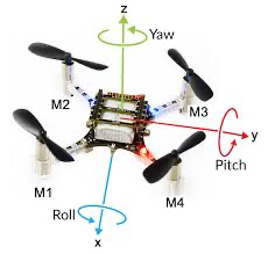
\includegraphics[width=0.6 \textwidth]{Relazione/Immagini/Crazyflie_assi.png}	
    \caption{Drone e relativo sistema di riferimento Body}
    \label{fig:Crazyflie_assi}
\end{figure}

Il nostro drone è un Crazyflie prodotto da BitCraze del tutto equivalente a quello mostrato sopra con l'aggiunta del fatto che sul nostro abbiamo montato anche una piattaforma nella parte superiore che permettesse il posizionamento dei marker, indispensabili per permettere l’individuazione del Drone da parte delle telecamere, e che mostreremo di seguito. 

\section*{Markers}
\addcontentsline{toc}{section}{Markers}

\begin{figure}[h]
    \centering
    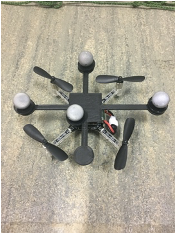
\includegraphics[width=0.6 \textwidth]{Relazione/Immagini/Markers.png}	
    \caption{Piattaforma per posizionamento Markers}
    \label{fig:Markers}
\end{figure}

Al fine di permettere la corretta individuazione del Drone da parte delle telecamere, abbiamo sviluppato un’apposita piattaforma che è stata poi stampata e apposta sulla parte superiore al fine di permettere un migliore posizionamento dei marker. Dato che marker troppo vicini davano fastidio al sistema di visione, abbiamo scelto una piattaforma che si estendesse maggiormente in ampiezza rispetto a quella originale grazie ai prolungamenti che riescono a passare tra le eliche senza dare loro fastidio durante il volo. Il colore nero è preferibile in quanto tra tutti è quello che meno riflette e che causa quindi minori interferenze con le telecamere. La disposizione dei maker è arbitraria purchè siano fissati in modo rigido e non crei una geometria simmetrica, ciò è necessario in quanto durante il movimento del Drone il sistema di visione deve poter riconoscere l’orientamento del Drone senza ambiguità, non si devono dunque verificare casi in cui la disposizione dei marker potrebbe corrispondere a due o più diverse configurazioni del Drone, in quel caso infatti il sistema non riuscirebbe a riconoscere l'orientazione corretta del Drone e fornirebbe quindi valori di orientazione errati rispetto a quelli reali. 

\section*{Eliche}
\addcontentsline{toc}{section}{Eliche}

\begin{figure}[h]
    \centering
    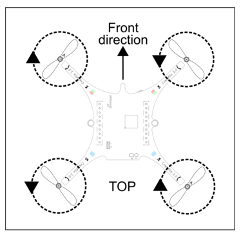
\includegraphics[width=0.6 \textwidth]{Relazione/Immagini/Eliche.png}	
    \caption{Corretto posizionamento delle eliche}
    \label{fig:Eliche}
\end{figure}

Dato che può capitare che un esperimento non vada come previsto e termini con una caduta del Drone, una breve parentesi sul corretto montaggio delle eliche è necessaria in quanto potrebbe succedere che nella caduta alcune si stacchino dal relativo albero. 
Nel caso in qui questo succeda è necessario tenere a mente che le eliche sono di due tipi e che, come indica la figura, il montaggio non è del tutto arbitrario ma deve seguire la seguente logica: 
\begin{itemize}
    \item \verb Eliche  \verb di  \verb tipo  \verb A2:  queste devono essere montate sui motori il cui verso di rotazione è quello orario. 
    \item \verb Eliche  \verb di  \verb tipo  \verb B2:  al contrario, devono essere montate sui motori il cui verso di rotazione è quello  antiorario.
\end{itemize}

Si fa notare che le eliche dello stesso tipo saranno alla fine disposte l’una di fronte all’altra (non accanto) e che il verso di rotazione di ciascun motore è riportato sui terminali del drone come ultimo simbolo. \\ 
Nel momento in cui queste vengono rimontate è bene fare una pressione abbastanza forte in modo da assicurarsi che non si stacchino più con facilità. 

\section*{Crazyradio}
\addcontentsline{toc}{section}{Crazyradio}


\begin{figure}[h]
    \centering
    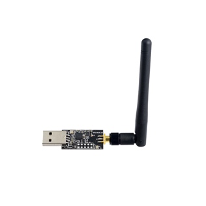
\includegraphics[width=0.4 \textwidth]{Relazione/Immagini/Crazyradio.png}
    \caption{Crazyradio}
    \label{fig:Crazyradio}
\end{figure}
\\
\\
\\
\\
\\
\\
\\
\\
\\
\\
\\
\\
\\
\\
\\
\\


Per poter comunicare il Drone utilizza il protocollo CRTP appositamente sviluppato da Bitcraze (verrà descritto nel dettaglio più avanti). \\ 
La Crazyradio è il mezzo che consente la comunicazione bidirezionale tra il pc su cui essa è installata e il Drone. 

\section*{Vicon Active Wand}
\addcontentsline{toc}{section}{Vicon Active Wand}

\begin{figure}[h]
    \centering
    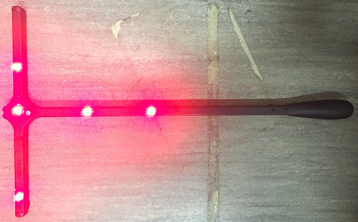
\includegraphics[width=0.5 \textwidth]{Relazione/Immagini/Wand.png}
    \caption{Vicon Active Wand in funzione}
    \label{fig:Wand}
\end{figure}

Questa è la “Bacchetta” da noi utilizzata come target da inseguire. Come si nota ha già installati dei piccoli laser che una volta accesi fungono da marker. A differenza dei marker del drone (passivi) questi sono marker attivi e dunque conenstono un tracciamento molto più preciso da parte delle telecamere. \\
A volte è anche utilizzata per ricalibrare l’intero sistema e fornire posizione e orientazione della terna fissa (da noi rinominata come  "terna Vicon"). La ricalibrazione è consigliata all'inizio di ogni sessione di esperimenti, in alternativa, ogni volta che si verificano cambiamenti in termini di "fantasie" di pavimentazione, luce, temperatura … Diventa praticamente obbligatoria invece nel momento in cui il Software non riesce a visualizzare correttamente i marker (attivi o passivi) posti sugli oggetti, può anche accadere che ne vengano mostrati più di quanti in realtà sono presenti sui relativi oggetti. 

\section*{Vicon Tracker}
\addcontentsline{toc}{section}{Vicon Tracker}

\begin{figure}[h]
    \centering
    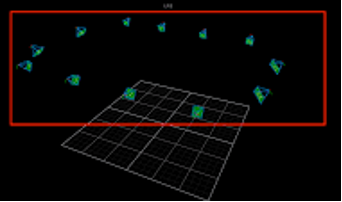
\includegraphics[width=0.6 \textwidth]{Relazione/Immagini/Tracker.png}
    \caption{Software Tracker in funzione con evidenziate in rosso le telecamere disposte nella flight room, il cui pavimento è rappresentato dalla griglia.}
    \label{fig:Tracker}
\end{figure}

Il Sistema di tracciamento Vicon è in realtà costituito sia da Hardware che da Software, più precisamente il Software di Tracking si avvale delle telecamere, posizionate nella flight room, per individuare i Markers posti sugli oggetti. \\
In figura si mostrano le telecamere così come appaiono dal software. \\
Inizialmente (e periodicamente) il sistema ha bisogno di una ricalibrazione grazie alla quale, con l'ausilio della Wand, viene fatto un reset delle impostazioni delle telecamere per renderle pù precise; vengono inoltre reimpostate sia l'origine della terna fissa (solitamente posta al centro della stanza) che l'orientazione dei relativi assi. \\
Una volta calibrato, il sistema deve essere in grado di individuare in modo esatto i markers piazzati sugli oggetti. Questi possono essere selezionati in gruppo per creare degli "oggetti software" da associare ai "dispositivi fisici". Tra le proprietà (campi) più utili di questi oggetti troviamo il nome, utilizzato come "alias" all'interno del codice Python, e i sistemi di riferimento "body", che devono essere opportunamente inzializzati con posizione e orientazione desiderati (in alternativa il sistema li inizializza nel modo che sul momento ritiene più adatto, è dunque sempre consigliato di reimpostarli manualmente). 